\documentclass[11pt]{article}
\usepackage{amsmath, amssymb, physics, mathtools, bm}
\usepackage{tikz, pgfplots}
\pgfplotsset{compat=1.18}
\usepackage[margin=2.3cm]{geometry}
\usepackage{siunitx, booktabs, hyperref}
\usepackage{braket}
\newcommand{\D}{\mathrm{D}}
\newcommand{\de}{\mathrm{d}}
\newcommand{\pd}[2]{\frac{\partial #1}{\partial #2}}
\newcommand{\pdd}[2]{\frac{\partial^{2} #1}{\partial #2^{2}}}
\newcommand{\Lap}{\nabla^{2}}
\title{B3 Atomic, Quantum and Laser Physics, 2025 --- Model Solutions}
\author{}
\date{}
\begin{document}
\maketitle

%==========================================================
\section*{Question 1 --- Two-electron atoms: Ca and Ba}

\textbf{Problem.} Ca ($Z=20$) and Ba ($Z=56$) level diagrams labelled X, Y; closed core $+$ two valence $s$ electrons. Identify, label, and discuss term/level structure and E1 transitions.

\subsection*{(a) Central-field approximation and configurations}

Exact Hamiltonian
\[
H = \sum_{i}\!\left(-\tfrac{\hbar^{2}}{2m_e}\Lap_i - \tfrac{Ze^{2}}{4\pi\epsilon_0 r_i}\right) + \sum_{i<j}\tfrac{e^{2}}{4\pi\epsilon_0 r_{ij}}
\]
is non-separable. Replace mean effect of other electrons by a spherical $V_c(r_i)$ interpolating between bare ($-Ze^2/4\pi\epsilon_0 r$) and fully screened ($-e^2/4\pi\epsilon_0 r$). Then
\begin{equation}
H_0 = \sum_i \left[-\tfrac{\hbar^{2}}{2m_e}\Lap_i + V_c(r_i)\right]
\label{eq:Hcf}
\end{equation}
separates; one-electron states carry $(n,\ell,m_\ell,m_s)$ with $\ell$-dependent energies (low-$\ell$ orbitals penetrate the core). Filling shells antisymmetrically by Pauli gives the \textbf{electron configuration} $(1s)^2(2s)^2\cdots$.

\subsection*{(b) Terms and levels}

$H_0$-degeneracy of a configuration is lifted by:
\begin{itemize}
\item Residual electrostatic $H_1$: commutes with $\vb L,\vb S$, so splits the configuration into LS \textbf{terms} $^{2S+1}\!L$. Exchange part favours high $S$ (Hund's first rule).
\item Spin--orbit $H_{SO}=\sum_i \zeta(r_i)\,\vb \ell_i\!\cdot\!\vb s_i$: couples $\vb L,\vb S\to\vb J$, splitting each term into \textbf{levels} $^{2S+1}\!L_J$, $J=|L-S|,\ldots,L+S$.
\end{itemize}
Light atoms: term-splitting $\gg$ fine structure (LS coupling). Heavy atoms drift toward $jj$.

\subsection*{(c) Identification}

Both have $(ns)^2$ ground giving $^1S_0$; lowest excited configurations are $ns(n-1)d$ and $nsnp$. In X, $ns(n-1)d$ lies \emph{below} $nsnp$ and the triplet fine structure ($\sim 10^3\,\si{cm^{-1}}$) is large enough to be visible directly; in Y the order is reversed and the fine structure is so small ($\sim 50\,\si{cm^{-1}}$) that a $\times 20$ inset is needed. In heavy atoms $(n-1)d$ is pulled in and fine structure $\sim Z^4\alpha^2$ is large, so
\begin{equation}
\boxed{\;\text{X = Ba}\,(Z=56),\qquad \text{Y = Ca}\,(Z=20).\;}
\label{eq:identify}
\end{equation}

\subsection*{(d) Term and level labels}

Closed $(ns)^2$:
\[
(ns)^{2}:\quad {}^{1}S_0.
\]
$nsnp$ ($\ell=0,1\Rightarrow L=1$; $S=0,1$):
\[
nsnp:\quad {}^{3}P_0,{}^{3}P_1,{}^{3}P_2,\;{}^{1}P_1.
\]
$ns(n-1)d$ ($\ell=0,2\Rightarrow L=2$; $S=0,1$):
\[
ns(n-1)d:\quad {}^{3}D_1,{}^{3}D_2,{}^{3}D_3,\;{}^{1}D_2.
\]
Ba: $6s^2$, $6s5d$, $6s6p$. Ca: $4s^2$, $4s3d$, $4s4p$. In each diagram the close-spaced triplet is the $^3P$ or $^3D$ multiplet; the isolated higher line is the singlet.

\subsection*{(e) Singlet--triplet ordering}

Triplet space part is antisymmetric, electrons avoid each other; singlet symmetric, electrons overlap, larger Coulomb. Exchange splitting
\begin{equation}
E({}^{1}L)-E({}^{3}L)=2K_{ns,n'\ell},\qquad K=\!\!\int\! \de^{3}r_1 \de^{3}r_2\,\psi_{ns}^{*}(1)\psi_{n'\ell}^{*}(2)\tfrac{e^{2}}{4\pi\epsilon_0 r_{12}}\psi_{n'\ell}(1)\psi_{ns}(2)>0.
\label{eq:exchange}
\end{equation}

\subsection*{(f) Interval rule}

$H_{SO}=A\,\vb L\!\cdot\!\vb S$ in $\ket{LSJM_J}$ gives Land\'e's
\begin{equation}
E_J - E_{J-1} = A\,J.
\label{eq:lande}
\end{equation}
Requires (i) pure LS, fine structure $\ll$ term splitting; (ii) one $A$ per term (single-configuration). Hence \emph{much better obeyed in Ca than Ba}: e.g.\ Ca $4s4p\,^3P$: $(E_2-E_1)/(E_1-E_0)\approx 1.96$ (cf.\ predicted 2); Ba $6s6p\,^3P$ ratio is significantly distorted.

\subsection*{(g) Allowed E1 transitions in Ba}

Selection rules: parity flip ($\Delta\ell=\pm 1$ on one electron); $\Delta S=0$; $\Delta L=0,\pm 1$ ($0\not\to 0$); $\Delta J=0,\pm 1$ ($0\not\to 0$). From $6s^2\,^1S_0$ only $6s6p\,^1P_1$ is reachable ($s\to d$ forbidden by parity, triplets by $\Delta S$). Within excited configurations:
\begin{align*}
\textbf{Resonance:}\;\; & 6s^{2}\,{}^{1}S_0 \to 6s6p\,{}^{1}P_1, \\
{}^{3}D\!\to\!{}^{3}P:\;\; & {}^{3}D_1\to{}^{3}P_{0,1,2};\;{}^{3}D_2\to{}^{3}P_{1,2};\;{}^{3}D_3\to{}^{3}P_2, \\
{}^{1}D\!\to\!{}^{1}P:\;\; & {}^{1}D_2 \to {}^{1}P_1.
\end{align*}
Strongest: \boxed{6s^{2}\,{}^{1}S_0 \leftrightarrow 6s6p\,{}^{1}P_1} resonance line: connects populated ground level, $\Delta S=0$ (no spin-forbidden suppression), largest $\omega^3$ in $A_{21}$ and large $\bra{6s}r\ket{6p}$.

%==========================================================
\section*{Question 2 --- Hydrogenic energy scales and positronium in a magnetic field}

\textbf{Problem.} (a) H gross/fine/hyperfine scales; (b) Ps Bohr levels and $\langle r_{ep}\rangle$; (c)--(e) eigenstates, good QNs, energies and sketch for $H=A\,\vb s_e\!\cdot\!\vb s_p+2\mu_B(\vb s_e-\vb s_p)\!\cdot\!\vb B$; (f) fine/hyperfine of Ps $p$-configurations.

\subsection*{(a) Energy scales}

Gross (Rydberg):
\begin{equation}
E_{\rm gross} \sim \tfrac12\, m_e c^{2}\alpha^{2}\;\;(\approx \SI{13.6}{eV}).
\end{equation}
Fine (relativistic, SO, Darwin), one extra $(v/c)^2\sim\alpha^2$:
\begin{equation}
E_{\rm fs} \sim m_e c^{2}\alpha^{4}\;\;(\approx \SI{e-4}{eV}).
\end{equation}
Hyperfine: nuclear $\mu_p\sim\mu_N\propto 1/m_p$ vs.\ $\mu_B\propto 1/m_e$, so suppressed by $m_e/m_p$:
\begin{equation}
E_{\rm hfs} \sim m_e c^{2}\alpha^{4}\,\frac{m_e}{m_p}\;\;(\approx \SI{e-7}{eV}).
\end{equation}
SO is electron magnetic moment in motional $B\sim\alpha^2 m_e^2 c^2/(e\hbar)$; hfs replaces one $\mu_B$ by $\mu_p$, hence ratio $m_e/m_p\approx 1/1836$.

\subsection*{(b) Bohr Ps}

Reduced mass $\mu=m_e/2$, so $E_n=-\mu c^2\alpha^2/(2n^2)=\tfrac12 E_n^{\rm H}$:
\begin{equation}
\boxed{\;|E_1^{\rm Ps}| = \tfrac12 \times \SI{13.6}{eV}\approx \SI{6.8}{eV}.\;}
\end{equation}
Relative-coordinate Bohr radius $a_{\rm rel}=\hbar/(\mu c\alpha)=2a_0$, hence
\begin{equation}
\boxed{\;\langle r_{ep}\rangle_{1s} \sim 2 a_0.\;}
\end{equation}

\subsection*{(c) Eigenstate count and good quantum numbers}

$2\times 2=$ \boxed{4 \text{ eigenstates}}.

Low field ($A\gg 2\mu_B B$): hyperfine dominates; good QNs $(S_{\rm tot},M_{S_{\rm tot}})$ with $S_{\rm tot}=0$ (para) or $1$ (ortho).

High field ($2\mu_B B\gg A$): Zeeman dominates; field couples to $\vb s_e-\vb s_p$ so $\vb S_{\rm tot}$ not conserved; good QNs $(m_{s_e},m_{s_p})$.

\subsection*{(d) Energies}

\paragraph{Zero field.} Square the total spin:
\[
\vb S_{\rm tot}^2 = (\vb s_e+\vb s_p)^2 = \vb s_e^2 + \vb s_p^2 + 2\,\vb s_e\!\cdot\!\vb s_p.
\]
Solve for the dot product:
\[
\vb s_e\!\cdot\!\vb s_p = \tfrac12\!\left(\vb S_{\rm tot}^2 - \vb s_e^2 - \vb s_p^2\right).
\]
Take expectation in $\ket{S_{\rm tot},M}$ with $s_e=s_p=\tfrac12$:
\[
\langle\vb s_e\!\cdot\!\vb s_p\rangle = \tfrac{\hbar^2}{2}\!\left[S_{\rm tot}(S_{\rm tot}+1) - \tfrac32\right].
\]
Evaluate the two cases:
\[
\langle\vb s_e\!\cdot\!\vb s_p\rangle = \begin{cases}+\tfrac14\hbar^2,& S_{\rm tot}=1\\ -\tfrac34\hbar^2,& S_{\rm tot}=0.\end{cases}
\]
Multiply by $A$:
\begin{equation}
\boxed{\;E^{(0)}_{S=1} = +\tfrac14 A\hbar^{2}\;\;(\times 3),\qquad E^{(0)}_{S=0} = -\tfrac34 A\hbar^{2};\quad \text{splitting } A\hbar^2.\;}
\label{eq:zerofield}
\end{equation}

\paragraph{High field.} Choose $\vb B = B\hat{\vb z}$ and the product basis $\ket{m_{s_e},m_{s_p}}$. Expand the Zeeman term:
\[
H_Z = 2\mu_B B\,(s_{ez}-s_{pz}).
\]
Act on the product basis:
\[
H_Z\ket{m_{s_e},m_{s_p}} = 2\mu_B B\,\hbar(m_{s_e}-m_{s_p})\ket{m_{s_e},m_{s_p}}.
\]
Decompose the hyperfine operator into $z$ and ladder pieces:
\[
\vb s_e\!\cdot\!\vb s_p = s_{ez}s_{pz} + \tfrac12(s_{e+}s_{p-}+s_{e-}s_{p+}).
\]
Drop off-diagonal ladder terms (suppressed by large Zeeman gap):
\[
\langle\vb s_e\!\cdot\!\vb s_p\rangle \to \hbar^2 m_{s_e}m_{s_p}.
\]
Add the two contributions for each product state:
\begin{equation}
\boxed{\;\begin{aligned}
\ket{\!\!\uparrow_e\uparrow_p}: &\;\; E = +\tfrac14 A\hbar^{2},\\
\ket{\!\!\downarrow_e\downarrow_p}: &\;\; E = +\tfrac14 A\hbar^{2},\\
\ket{\!\!\uparrow_e\downarrow_p}: &\;\; E = -\tfrac14 A\hbar^{2}+2\mu_B B\hbar,\\
\ket{\!\!\downarrow_e\uparrow_p}: &\;\; E = -\tfrac14 A\hbar^{2}-2\mu_B B\hbar.
\end{aligned}\;}
\label{eq:highfield}
\end{equation}
Stretched $\ket{\!\!\uparrow\uparrow},\ket{\!\!\downarrow\downarrow}$ unaffected ($s_e-s_p$ has $m=0$ on these).

\subsection*{(e) Sketch versus $B$}

\begin{center}
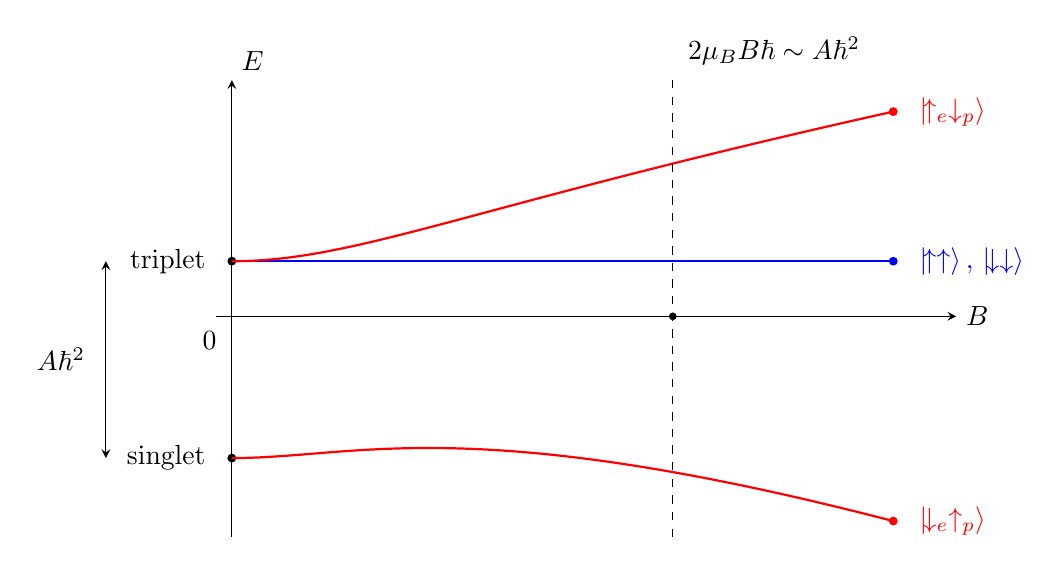
\begin{tikzpicture}[>=stealth, scale=1.0]
  % axes
  \draw[->] (0,-2.8) -- (0,3.0) node[above right] {$E$};
  \draw[->] (-0.2,0) -- (9.2,0) node[right] {$B$};
  \node[below left=2pt] at (0,0) {$0$};

  % zero-field anchor markers (filled circles outside any line label)
  \fill (0,0.7) circle (1.6pt);
  \fill (0,-1.8) circle (1.6pt);

  % zero-field labels at LEFT, energies/states at RIGHT (outside curves)
  \node[left=6pt] at (0,0.7)  {triplet};
  \node[left=6pt] at (0,-1.8) {singlet};

  % flat triplet stretched states (m=0 under (s_e - s_p))
  \draw[thick,blue] (0,0.7) -- (8.4,0.7);
  \fill[blue] (8.4,0.7) circle (1.6pt);
  \node[blue, right=6pt] at (8.4,0.7) {$\ket{\!\uparrow\uparrow},\,\ket{\!\downarrow\downarrow}$};

  % field-mixed branches (anti-cross): up_e down_p rises, down_e up_p falls
  \draw[thick,red] (0,0.7) .. controls (1.6,0.7) and (3.0,1.4) .. (8.4,2.6);
  \fill[red] (8.4,2.6) circle (1.6pt);
  \node[red, right=6pt] at (8.4,2.6) {$\ket{\!\uparrow_e\downarrow_p}$};

  \draw[thick,red] (0,-1.8) .. controls (1.6,-1.8) and (3.0,-1.2) .. (8.4,-2.6);
  \fill[red] (8.4,-2.6) circle (1.6pt);
  \node[red, right=6pt] at (8.4,-2.6) {$\ket{\!\downarrow_e\uparrow_p}$};

  % zero-field splitting bracket — placed outside the y-axis (to the left)
  \draw[<->] (-1.6,0.7) -- (-1.6,-1.8);
  \node[left=4pt] at (-1.6,-0.55) {$A\hbar^{2}$};

  % crossover marker
  \draw[dashed] (5.6,-2.8) -- (5.6,3.0);
  \fill (5.6,0) circle (1.4pt);
  \node[above right=2pt] at (5.6,3.0) {$2\mu_B B\hbar \sim A\hbar^{2}$};
\end{tikzpicture}
\end{center}

Crossover at $B^*=A\hbar/(2\mu_B)$; high-field slopes $\pm 2\mu_B\hbar$.

\subsection*{(f) Fine vs.\ hyperfine in Ps}

In Ps the ``nucleus'' has $m_p\to m_e$, so the $m_e/m_p$ suppression vanishes: \emph{fine and hyperfine merge at} $\sim m_e c^2\alpha^4\sim 10^{-4}\,\si{eV}$. For $\ell=1$ Ps: $^1P_1$ (para), $^3P_{0,1,2}$ (ortho), with SO + spin--spin (contact + tensor) all of the same order. Additional Ps-only contribution: virtual $e^+e^-$ annihilation into a virtual photon shifts $S_{\rm tot}=1$ levels at the same $\alpha^4$ order. The fine/hyperfine separation loses meaning here.

%==========================================================
\section*{Question 3 --- Two-level Rabi oscillations and inhomogeneous broadening}

\textbf{Problem.} Two-level atom in $\vb E=\mathcal E_0\cos(\omega t)\hat{\vb z}$ for time $T$; given
\begin{equation}
|c_2(T)|^{2} = \frac{\Omega^{2}}{\Omega^{2}+\delta^{2}}\sin^{2}\!\left(\tfrac12\sqrt{\Omega^{2}+\delta^{2}}\,T\right).
\label{eq:rabiformula}
\end{equation}

\subsection*{(a) $\Omega$ and $\delta$}

\begin{equation}
\boxed{\;\Omega = \frac{e\mathcal E_0}{\hbar}\,\bra{2}\hat z\ket{1} \equiv \frac{\mathcal E_0\, d_{12}}{\hbar},\qquad \delta=\omega-\omega_0,\quad \omega_0=\frac{E_2-E_1}{\hbar}.\;}
\end{equation}

\subsection*{(b) Assumptions}

(1) Two-level: other states off-resonance, $|\delta_{\rm other}|\gg\Omega$. (2) Electric dipole: $ka\ll 1$, i.e.\ $\lambda\gg a_0$. (3) Semi-classical field (large photon number, no spontaneous emission). (4) No spontaneous decay, $T\ll\tau$. (5) RWA: drop counter-rotating $e^{\pm 2i\omega t}$, valid for $\Omega,|\delta|\ll\omega,\omega_0$. (6) Initial condition $c_1(0)=1$, $c_2(0)=0$.

\subsection*{(c) Sketches}

\begin{center}
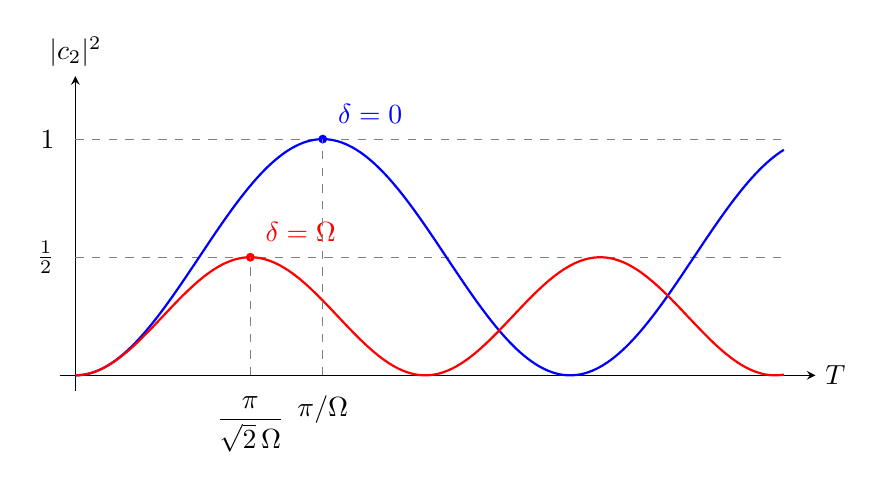
\begin{tikzpicture}[>=stealth, scale=1.0]
  % axes with labels at arrowhead ends
  \draw[->] (-0.2,0) -- (9.4,0) node[right] {$T$};
  \draw[->] (0,-0.2) -- (0,3.8) node[above] {$|c_2|^{2}$};

  % horizontal reference levels (dashed) with labels OUTSIDE on the left
  \draw[dashed,gray] (0,3.0) -- (9.0,3.0);
  \node[left=4pt] at (0,3.0) {$1$};
  \draw[dashed,gray] (0,1.5) -- (9.0,1.5);
  \node[left=4pt] at (0,1.5) {$\tfrac12$};

  % delta = 0 curve (full amplitude)
  \draw[thick,blue,domain=0:9.0,samples=200]
        plot (\x, {3*sin(0.5*\x*180/pi)*sin(0.5*\x*180/pi)});

  % delta = Omega curve (half amplitude, faster)
  \draw[thick,red,domain=0:9.0,samples=200]
        plot (\x, {1.5*sin(0.5*sqrt(2)*\x*180/pi)*sin(0.5*sqrt(2)*\x*180/pi)});

  % first-peak markers + curve labels parked OUTSIDE the curves
  \fill[blue] ({pi},3.0) circle (1.6pt);
  \node[blue, above right=2pt] at ({pi},3.0) {$\delta=0$};

  \fill[red] ({pi/sqrt(2)},1.5) circle (1.6pt);
  \node[red, above right=2pt] at ({pi/sqrt(2)},1.5) {$\delta=\Omega$};

  % x-axis tick marks for the two periods, labels BELOW the axis
  \draw[dashed,gray] ({pi},0)--({pi},3.0);
  \node[below=4pt] at ({pi},0) {$\pi/\Omega$};

  \draw[dashed,gray] ({pi/sqrt(2)},0)--({pi/sqrt(2)},1.5);
  \node[below=4pt] at ({pi/sqrt(2)},0) {$\dfrac{\pi}{\sqrt2\,\Omega}$};
\end{tikzpicture}
\end{center}

$\delta=0$: $|c_2|^2=\sin^2(\Omega T/2)$, full inversion at $T=\pi/\Omega$. $\delta=\Omega$: amplitude $\tfrac12$, period $2\pi/(\sqrt 2\Omega)$, first peak at $T=\pi/(\sqrt 2\Omega)$.

\subsection*{(d) Short-time limit}

For $\sqrt{\Omega^2+\delta^2}\,T\ll 1$, apply $\sin x\approx x$:
\[
\sin^{2}\!\left(\tfrac12\sqrt{\Omega^{2}+\delta^{2}}\,T\right) \approx \tfrac14(\Omega^{2}+\delta^{2})\,T^{2}.
\]
Multiply by the prefactor:
\[
|c_2(T)|^{2} \approx \frac{\Omega^{2}}{\Omega^{2}+\delta^{2}}\cdot\tfrac14(\Omega^{2}+\delta^{2})\,T^{2}.
\]
Cancel $(\Omega^2+\delta^2)$:
\begin{equation}
|c_2(T)|^{2} \approx \frac{(\Omega T)^{2}}{4},
\label{eq:smallT}
\end{equation}
\emph{independent of $\delta$}: time--energy uncertainty $\sim 1/T$ exceeds $\delta$, so all detunings within the pulse bandwidth are excited equally. Condition: $T\ll 1/\sqrt{\Omega^2+\delta^2}$.

\subsection*{(e) On-resonance $\pi$-pulse}

\begin{equation}
\boxed{\;T_\pi = \frac{\pi}{\Omega}.\;}
\label{eq:Tpi}
\end{equation}

\subsection*{(f) Ensemble average, $\Delta\ll\Omega$}

Substitute $T=T_\pi=\pi/\Omega$ into \eqref{eq:rabiformula}:
\[
P_2(\delta) = \frac{\Omega^{2}}{\Omega^{2}+\delta^{2}}\sin^{2}\!\left(\tfrac{\pi}{2}\sqrt{1+\delta^{2}/\Omega^{2}}\right).
\]
Binomial expand the prefactor:
\[
\frac{\Omega^{2}}{\Omega^{2}+\delta^{2}} = \frac{1}{1+\delta^{2}/\Omega^{2}} \approx 1 - \frac{\delta^{2}}{\Omega^{2}} + \mathcal O(\delta^{4}/\Omega^{4}).
\]
Expand the square root to first order:
\[
\sqrt{1+\delta^{2}/\Omega^{2}} \approx 1 + \frac{\delta^{2}}{2\Omega^{2}}.
\]
The sine argument becomes
\[
\frac{\pi}{2}\sqrt{1+\delta^{2}/\Omega^{2}} \approx \frac{\pi}{2} + \frac{\pi\delta^{2}}{4\Omega^{2}}.
\]
Apply the identity $\sin(\pi/2+x)=\cos x$:
\[
\sin^{2}\!\left(\tfrac{\pi}{2} + \tfrac{\pi\delta^{2}}{4\Omega^{2}}\right) = \cos^{2}\!\left(\tfrac{\pi\delta^{2}}{4\Omega^{2}}\right).
\]
Cosine to second order:
\[
\cos\!\left(\tfrac{\pi\delta^{2}}{4\Omega^{2}}\right) \approx 1 - \tfrac{1}{2}\!\left(\tfrac{\pi\delta^{2}}{4\Omega^{2}}\right)^{2} = 1 + \mathcal O(\delta^{4}/\Omega^{4}).
\]
Square it:
\[
\cos^{2}\!\left(\tfrac{\pi\delta^{2}}{4\Omega^{2}}\right) = 1 + \mathcal O(\delta^{4}/\Omega^{4}).
\]
Combine with the prefactor:
\[
P_2(\delta) \approx \left(1 - \tfrac{\delta^{2}}{\Omega^{2}}\right)\!\left(1 + \mathcal O(\delta^{4}/\Omega^{4})\right) = 1 - \frac{\delta^{2}}{\Omega^{2}}.
\]
Take the ensemble mean over uniform $\delta\in[-\Delta/2,\Delta/2]$:
\[
\langle\delta^2\rangle = \frac{1}{\Delta}\int_{-\Delta/2}^{\Delta/2}\!\delta^2\,\de\delta = \frac{\Delta^2}{12}.
\]
Insert into $\langle P_2\rangle$:
\begin{equation}
\boxed{\;\langle P_2\rangle = 1 - \frac{1}{12}\!\left(\frac{\Delta}{\Omega}\right)^{2}.\;}
\label{eq:Pavg}
\end{equation}
Impose $\langle P_2\rangle > 0.99$:
\[
1 - \frac{1}{12}\!\left(\frac{\Delta}{\Omega}\right)^{2} > 0.99.
\]
Rearrange:
\[
\frac{\Delta^{2}}{12\,\Omega^{2}} < 0.01.
\]
Solve for $\Omega/\Delta$:
\[
\left(\frac{\Omega}{\Delta}\right)^{2} > \frac{1}{0.12} \approx 8.33.
\]
\begin{equation}
\boxed{\;\Omega/\Delta \gtrsim 2.9.\;}
\end{equation}

\subsection*{(g) Long-time limit}

$\sqrt{\Omega^2+\delta^2}\,T\gg 1$: $\sin^2$ averages to $\tfrac12$. With $\Omega\gg\Delta$ prefactor $\to 1$. Hence
\begin{equation}
\boxed{\;\langle P_2\rangle \to \frac{1}{2}.\;}
\end{equation}
Dephasing across the ensemble ($\Delta T\gg 1$) destroys the coherent oscillation; ``half-saturated'' incoherent steady state.

%==========================================================
\section*{Question 4 --- Line broadening, saturation and Doppler-free spectroscopy}

\textbf{Problem.} (a) Homogeneous vs.\ inhomogeneous; (b)--(d) rate equation, $\de I/\de z$ in saturated form, identify $\kappa,I_s$; (e)--(f) sketch $^{85}$Rb cell ($L=10\,$cm, $N_T=10^8\,\si{cm^{-3}}$, $\lambda_0=780\,$nm, $\tau=27\,$ns, $\sigma_{\rm peak}=3\times 10^{-9}\,\si{cm^2}$) at $1\,$mK and $10\,$K, then add saturating counter-pump.

\subsection*{(a) Homogeneous vs.\ inhomogeneous}

\textbf{Homogeneous}: every atom has the same broadened line. Examples: natural (Lorentzian, FWHM $\Gamma=1/\tau$); pressure/collisional. \textbf{Inhomogeneous}: different atoms have different transition frequencies; ensemble line is convolution of single-atom line with the distribution. Example: Doppler (Gaussian). Inhomogeneous broadening can be undone (saturation spectroscopy, photon echoes); homogeneous cannot.

\subsection*{(b) Rate equation}

\begin{equation}
\frac{\de N_2}{\de t} = (N_1-N_2)\,\sigma(\omega-\omega_0)\,\frac{I}{\hbar\omega} - \frac{N_2}{\tau}.
\label{eq:rateN2}
\end{equation}

\subsection*{(c) Absorbed power and Beer-like equation}

Spontaneous emission radiates into $4\pi$, not the beam, so only net stimulated processes attenuate $I$:
\[
\mathcal P_{\rm abs} = (N_1-N_2)\,\sigma(\omega-\omega_0)\,I \equiv \Delta N\,\sigma(\omega-\omega_0)\,I.
\]
\begin{equation}
\boxed{\;\frac{\de I}{\de z} = -\Delta N\,\sigma(\omega-\omega_0)\,I.\;}
\label{eq:dIdz}
\end{equation}

\subsection*{(d) Steady-state imbalance and saturation}

Set $\de N_2/\de t=0$ in \eqref{eq:rateN2}:
\[
(N_1-N_2)\,\sigma\,\frac{I}{\hbar\omega} = \frac{N_2}{\tau}.
\]
Define the dimensionless intensity $s=\sigma I\tau/(\hbar\omega)$:
\[
N_2 = (N_1-N_2)\,s.
\]
Expand and collect $N_2$:
\[
N_2(1+s) = N_1 s.
\]
Solve for $N_2$ in terms of $N_1$:
\[
N_2 = \frac{s}{1+s}\,N_1.
\]
Use total population $N_1+N_2=N_T$ with $N_1 = N_T - N_2$:
\[
N_2(1+s) = (N_T-N_2)\,s.
\]
Collect $N_2$ again:
\[
N_2(1+2s) = N_T s.
\]
Solve for the populations:
\[
N_1 = \frac{1+s}{1+2s}\,N_T,\qquad N_2 = \frac{s}{1+2s}\,N_T.
\]
Form the imbalance $\Delta N = N_1-N_2$:
\[
\Delta N = \frac{N_T}{1+2s}.
\]
Substitute into \eqref{eq:dIdz}:
\[
\frac{\de I}{\de z} = -\frac{N_T\,\sigma\,I}{1+2s}.
\]
Identify $2s = I/I_s$ with $I_s = \hbar\omega/(2\sigma\tau)$:
\begin{equation}
\frac{\de I}{\de z} = -\frac{N_T\sigma\,I}{1+I/I_s},\qquad
\boxed{\;\kappa(\omega) = N_T\,\sigma(\omega-\omega_0),\qquad I_s(\omega) = \frac{\hbar\omega}{2\,\sigma(\omega-\omega_0)\,\tau}.\;}
\label{eq:kappaIs}
\end{equation}
At $I=I_s$, $\Delta N$ halves and absorption halves; factor 2 because each absorption depletes $N_1$ and adds to $N_2$.

\subsection*{(e) Weak-beam profiles}

For $I\ll I_s$, $1+I/I_s\to 1$, so the saturated equation reduces to the linear Beer form. Separate variables:
\[
\frac{\de I}{I} = -N_T\,\sigma\,\de z.
\]
Integrate from $0$ to $z$:
\[
\ln I(z) - \ln I_0 = -N_T\,\sigma\,z.
\]
Exponentiate:
\[
I(z) = I_0\,\exp[-N_T\,\sigma\,z],
\]
so $I(L)=I_0\exp[-N_T\sigma L]$.

\textbf{Natural FWHM:} $\Delta\nu_{\rm nat}=1/(2\pi\tau)\approx \SI{5.9}{MHz}$.

\textbf{Doppler FWHM:} with $m=85\,m_u=\SI{1.41e-25}{kg}$, $\lambda_0=\SI{780}{nm}$,
\[
\Delta\nu_D = \frac{1}{\lambda_0}\sqrt{\frac{8 k_B T \ln 2}{m}}.
\]
Plug in $T=\SI{10}{K}$:
\[
\Delta\nu_D(\SI{10}{K}) = \frac{1}{\SI{780e-9}{m}}\sqrt{\frac{8\times\SI{1.38e-23}{J/K}\times \SI{10}{K}\times \ln 2}{\SI{1.41e-25}{kg}}}.
\]
Reduce the radical:
\[
\Delta\nu_D(\SI{10}{K}) \approx \frac{\SI{73.7}{m/s}}{\SI{780e-9}{m}} \approx \SI{94}{MHz}.
\]
Scale by $\sqrt{T}$ (factor $10^{-2}$) to get $T=\SI{1}{mK}$:
\[
\Delta\nu_D(\SI{1}{mK})\approx \SI{0.94}{MHz}.
\]

At $\SI{1}{mK}$: Doppler ($\SI{0.94}{MHz}$) $\ll$ natural ($\SI{5.9}{MHz}$), so the line is natural-dominated Lorentzian, FWHM $\approx \SI{5.9}{MHz}$, $\sigma\approx\sigma_{\rm peak}$. Compute optical depth:
\[
N_T\sigma L \approx 10^{8}\,\si{cm^{-3}}\times 3\times 10^{-9}\,\si{cm^{2}}\times 10\,\si{cm} = 3.
\]
On-resonance transmission:
\[
e^{-3}\approx 5\%.
\]

At $\SI{10}{K}$: Doppler ($\SI{94}{MHz}$) $\gg$ natural ($\SI{5.9}{MHz}$), so the line is Doppler-dominated Gaussian, FWHM $\approx \SI{94}{MHz}$. Peak $\sigma$ reduced by $\Gamma_{\rm nat}/\Delta\omega_D$:
\[
\sigma_{\rm peak}^{\rm eff}/\sigma_{\rm peak} \approx \SI{5.9}{MHz}/\SI{94}{MHz} \approx 0.063.
\]
Compute optical depth:
\[
N_T\sigma L \approx 3\times 0.063 \approx 0.19.
\]
On-resonance transmission:
\[
e^{-0.19}\approx 83\%.
\]

\begin{center}
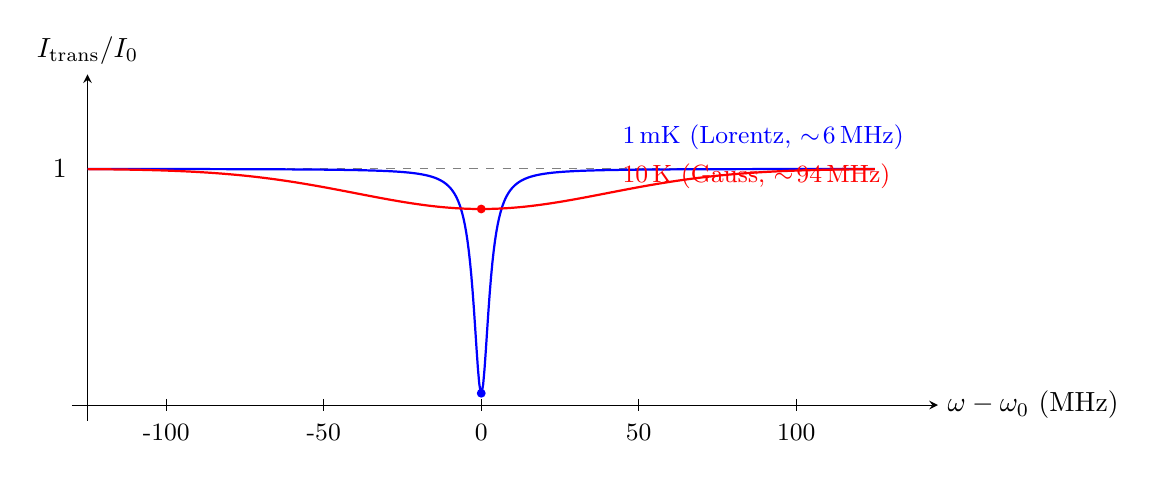
\begin{tikzpicture}[>=stealth, scale=1.0]
  % axes with labels at arrowhead ends
  \draw[->] (-0.2,0) -- (10.8,0) node[right] {$\omega-\omega_0$ (MHz)};
  \draw[->] (0,-0.2) -- (0,4.2) node[above] {$I_{\rm trans}/I_0$};

  % unity transmission level
  \draw[dashed,gray] (0,3.0)--(10.0,3.0);
  \node[left=4pt] at (0,3.0) {$1$};

  % T = 1 mK : narrow Lorentz, deep dip (FWHM ~6 MHz = 0.24 tikz units)
  \draw[thick,blue,domain=0:10,samples=600]
       plot (\x, {3 - 2.85/(1+((\x-5)/0.12)^2)});

  % T = 10 K : broad Gauss, shallow dip
  \draw[thick,red,domain=0:10,samples=240]
       plot (\x, {3 - 0.51*exp(-((\x-5)/3.76)^2*ln(2)*4)});

  % anchor markers + labels OUTSIDE the curves (above the trace, parked right)
  \fill[blue] (5,0.15) circle (1.6pt);
  \node[blue, above right=2pt] at (6.6,3.05) {\small $\SI{1}{mK}$ (Lorentz, $\sim\!\SI{6}{MHz}$)};

  \fill[red] (5,2.49) circle (1.6pt);
  \node[red, above right=2pt] at (6.6,2.55) {\small $\SI{10}{K}$ (Gauss, $\sim\!\SI{94}{MHz}$)};

  % x-axis tick marks; numeric labels BELOW the axis (outside)
  \foreach \x/\v in {1/-100,3/-50,5/0,7/50,9/100} {
    \draw (\x,0.08)--(\x,-0.08);
    \node[below=2pt] at (\x,-0.05) {\small \v};
  }
\end{tikzpicture}
\end{center}

\subsection*{(f) Doppler-free saturation at $\SI{10}{K}$}

Counter-propagating pump at $\omega_0$, $I_p\sim I_s$. Atom of velocity $v_z$ sees probe at $\omega(1+v_z/c)$, pump at $\omega_0(1-v_z/c)$. Pump saturates only $v_z=0$ atoms; probe is on resonance with that class only at $\omega=\omega_0$. A narrow \textbf{Lamb dip} (here, a peak in transmission) of width $\sim\Gamma_{\rm nat}\approx \SI{6}{MHz}$ appears at line centre on the broad Doppler dip:

\begin{center}
\begin{tikzpicture}[>=stealth, scale=1.0]
  % axes with labels at arrowhead ends
  \draw[->] (-0.2,0) -- (10.8,0) node[right] {$\omega-\omega_0$ (MHz)};
  \draw[->] (0,-0.2) -- (0,4.2) node[above] {$I_{\rm trans}/I_0$};

  % unity transmission level
  \draw[dashed,gray] (0,3.0)--(10.0,3.0);
  \node[left=4pt] at (0,3.0) {$1$};

  % broad Doppler dip (probe alone)
  \draw[thick,red,domain=0:10,samples=240]
       plot (\x, {3 - 0.51*exp(-((\x-5)/3.76)^2*ln(2)*4)});

  % broad dip + narrow Lamb peak at line centre (FWHM ~6 MHz)
  \draw[thick,green!55!black,domain=0:10,samples=600]
       plot (\x, {3 - 0.51*exp(-((\x-5)/3.76)^2*ln(2)*4)
                    + 0.35/(1+((\x-5)/0.12)^2)});

  % anchor markers and labels — both parked OUTSIDE their curves
  \fill[green!55!black] (5,2.84) circle (1.6pt);
  \node[green!55!black, above right=2pt] at (6.0,3.05)
       {\small with pump (Lamb dip)};

  \fill[red] (5,2.49) circle (1.6pt);
  \node[red, above right=2pt] at (6.0,2.20)
       {\small without pump};

  % x-axis tick marks with numeric labels parked BELOW
  \foreach \x/\v in {1/-100,3/-50,5/0,7/50,9/100} {
    \draw (\x,0.08)--(\x,-0.08);
    \node[below=2pt] at (\x,-0.05) {\small \v};
  }
\end{tikzpicture}
\end{center}

This is \textbf{Doppler-free saturation spectroscopy}: removes inhomogeneous broadening at the cost of a strong pump.

\end{document}
